\documentclass[border=5pt]{standalone}
\usepackage{tikz}

\begin{document}
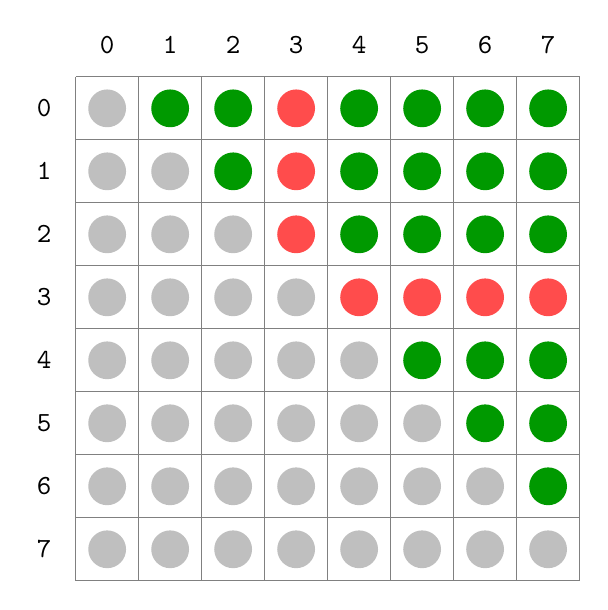
\begin{tikzpicture}[scale=0.8]

  % Grid
  \draw[step=1cm,gray,thin] (0,0) grid (8,8);

  % Column headers
  \foreach \x in {0,...,7} {
    \node at (\x+0.5, 8.5) {\texttt{\x}};
  }

  % Row headers
  \foreach \y in {0,...,7} {
    \pgfmathtruncatemacro{\label}{7-\y}
    \node at (-0.5, \y+0.5) {\texttt{\label}};
  }

  % Draw circles
  \foreach \row in {0,...,7} {
    \foreach \col in {0,...,7} {
      \pgfmathtruncatemacro{\y}{7-\row}

      % Diagonal and below - grey
      \ifnum\col<\row
        \fill[gray!50] (\col+0.5, \y+0.5) circle (0.3cm);
      \fi
      \ifnum\col=\row
        \fill[gray!50] (\col+0.5, \y+0.5) circle (0.3cm);
      \fi

      % Player 3 pairs (row 3 or column 3, above diagonal) - red
      \ifnum\col>\row
        \ifnum\row=3
          \fill[red!70] (\col+0.5, \y+0.5) circle (0.3cm);
        \else
          \ifnum\col=3
            \fill[red!70] (\col+0.5, \y+0.5) circle (0.3cm);
          \else
            % Other available pairs - green
            \fill[green!60!black] (\col+0.5, \y+0.5) circle (0.3cm);
          \fi
        \fi
      \fi
    }
  }

\end{tikzpicture}
\end{document}
